

\documentclass[11pt, draftclsnofoot, onecolumn]{IEEEtran} 

\usepackage{epsfig}
\usepackage{times}
\usepackage{subfigure}
\usepackage{amsfonts}
\usepackage{amsmath}
\usepackage{amssymb}
\usepackage{graphicx}
\usepackage{url}
%\usepackage{cite}
\usepackage{psfrag}
%\usepackage{stfloats}
\usepackage{array}
\usepackage{mdwmath} % part of Mark Wooding's powerful
\usepackage{mdwtab}  % tools for math, tables, ...
\usepackage{multirow}
\usepackage{verbatim}
\usepackage{wrapfig}
%\usepackage{booktabs}
%\usepackage{rotating}
\usepackage{color}
%\usepackage{upgreek}
%\usepackage{setspace}
%\usepackage{afterpage}

\newtheorem{thm}{Theorem}
\newtheorem{cor}[thm]{Corollary}
\newtheorem{lem}[thm]{Lemma}
\newtheorem{dfn}{Definition}
\newtheorem{pbm}{Problem}
\newtheorem{claim}{Claim}

\catcode`"=\active
\gdef"#1"{{\sf #1}}

\newcommand{\handout}[2]{
University of Texas at Austin\hfill{#2}
\newline
Department of Computer Science
\newline
Probabilistic Methods, Spring 1992
\newline
Handout \##1
\newline
}

\newcommand{\lecture}[4]{
University of Texas at Austin\hfill{#2}
\newline
Department of Computer Science
\newline
Probabilistic Methods, Spring 1992\hfill Lecturer: {#3}
\newline
Lecture \##1\hfill Scribe: {#4}
\newline
}

%\setlength{\parskip}{0.85ex}
%\setlength{\parindent}{0pt}

\newcommand{\id}[1]{{\it #1}}

\newcommand{\Eqnum}[1]{(\ref{eqn:#1})}
\newcommand{\Eqn}[1]{Equation~\Eqnum{#1}}
\newtheorem{Convention}{Convention}
\newtheorem{Definition}{Definition}
\newtheorem{Theorem}{Theorem}
\newtheorem{Example}{Example}[section]
\newtheorem{Remark}{Remark}
\newtheorem{Notation}{Notation}
\newtheorem{F}{Fact}
\newtheorem{Lemma}{Lemma}
\newtheorem{Corol}{Corollary}[Theorem]
\newtheorem{Lcorol}{Corollary}[Lemma]
\newtheorem{Proposition}{Proposition}

%\newenvironment{Proof}{\noindent{\bf Proof: }}{\hfill$\Box$}
\newenvironment{Invariant}[1]{\begin{quote}{Invariant\em#1\/}:}{\end{quote}}
%\newenvironment{Convention}[1]{\begin{quote}{Convention\em#1\/}:}{\end{quote}}
%\newcommand{\qed}{\protect\raisebox{.3ex}{\framebox[.5em]{\rule{0em}{.6ex}}}}

%\newcommand{\qed}{\nobreak \ifvmode \relax \else
%\ifdim\lastskip<1.5em \hskip-\lastskip
%\hskip1.5em plus0em minus0.5em \fi \nobreak
%\vrule height0.75em width0.5em depth0.25em\fi}

%%%% another environment for proof
%\newenvironment{proof}[1][Proof]{\begin{trivlist}
%\item[\hskip \labelsep {\bfseries #1}]}{\end{trivlist}}
%\newenvironment{definition}[1][Definition]{\begin{trivlist}
%\item[\hskip \labelsep {\bfseries #1}]}{\end{trivlist}}
%\newenvironment{example}[1][Example]{\begin{trivlist}
%\item[\hskip \labelsep {\bfseries #1}]}{\end{trivlist}}
%\newenvironment{remark}[1][Remark]{\begin{trivlist}
%\item[\hskip \labelsep {\bfseries #1}]}{\end{trivlist}}


\newcommand{\equals}{\stackrel{\rm def}{=}}
\newcommand{\ceil}[1]{\left\lceil  #1 \right\rceil}
\newcommand{\floor}[1]{\left\lfloor  #1 \right\rfloor}

\newcommand{\bin}[2]{\mathop{\mbox{\rm bin}}(#1,#2)}
\newcommand{\smallbin}[2]{\mathop{\mbox{\scriptsize{\rm bin}}}(#1,#2)}
\newcommand{\expectation}[1]{\mathop{\mbox{\rm E}}(#1)}
\newcommand{\variance}[1]{\mathop{\mbox{\rm Var}}(#1)}
\newcommand{\covariance}[2]{\mathop{\mbox{\rm Cov}}(#1,#2)}

\newcommand{\polyTime}{{\bf P }}
\newcommand{\NP}{{\bf NP }}
\newcommand{\coNP}{{\bf co-NP }}
\newcommand{\PSPACE}{{\bf PSPACE }}
\newcommand{\RNC}{{\bf RNC }}
\newcommand{\R}{{\bf R }}
\newcommand{\RP}{{\bf RP }}
\newcommand{\coR}{{\bf co-R }}
\newcommand{\coRP}{{\bf co-RP }}
\newcommand{\ZPP}{{\bf ZPP }}
\newcommand{\BPP}{{\bf BPP }}
\newcommand{\PP}{{\bf PP }}

\newcommand{\Iff}{\leftrightarrow}
\newcommand{\IFF}{\Longleftrightarrow}
\newcommand{\imp}{\rightarrow}
\newcommand{\Imp}{\Rightarrow}
\newcommand{\IMP}{\Longrightarrow}

\newcommand{\ints}{{\bf Z}}
\newcommand{\nats}{{\bf N}}
\newcommand{\reals}{{\bf R}}
\newcommand{\nTuples}{\ints^n}


%\renewcommand{\algorithmiccomment}[1]{/* #1 */}
%\renewcommand{\algorithmicloop}{\textbf{begin}}
%\renewcommand{\algorithmicendloop}{\textbf{end}}

\def\>{\hspace{0.27cm}}
%\def\>{\hspace{0.3cm}}
%\def\>{\hspace{0.5cm}}
%\def\^{\vspace{-0.5cm}}
\newcommand{\seprule}{\centerline{\rule{\linewidth}{0.3pt}\vspace{.1in}}}
\newcommand{\seprulelast}{\vspace{-0.1in}\centerline{\rule{\linewidth}{0.3pt}\vspace{-0.1in}}}


\newcommand{\Algorithm}[1]{\bigskip\noindent{\bf Algorithm }
        {#1}\vspace{-2mm}\par\nobreak}
\newcommand{\Protocol}[1]{\bigskip\noindent{}
        {\large \sf \bf {#1}}\vspace{.25cm}\par\nobreak}

\def\bs{\boldsymbol}

\def\bbegin{{\bf begin }} 
\def\bbreak{{\bf break}} 
\def\bfor{{\bf for }} 
\def\bstep{{\bf step }}
\def\bdo{{\bf do }}
\def\bgoto{{\bf goto }}
\def\bif{{\bf if }} 
\def\bfi{{\bf fi}}
\def\bthen{{\bf then }} 
\def\belse{{\bf else }}
\def\belsif{{\bf elsif }}
\def\belif{{\bf elif }}
\def\belseif{{\bf elif }}
\def\bboolean{{\bf boolean }}
\def\bwhile{{\bf while }}
\def\bendwhile{{\bf end while}}
\def\brepeat{{\bf repeat }}
\def\btimes{{\bf times}}
\def\buntil{{\bf until }}
\def\bend{{\bf end }} 
\def\bendif{{\bf end if }} 
\def\band{{\bf and }} 
\def\bor{{\bf or }} 
\def\bcor{{\bf cor }} 
\def\bcand{{\bf cand }} 
\def\bco{{\bf co }} 
\def\boc{{\bf oc}} 
\def\bod{{\bf od}}
\def\bto{{\bf to }}
\def\bdownto{{\bf downto }}
\def\balgorithm{{\bf algorithm }}
\def\bprocedure{{\bf procedure }}
\def\bfunction{{\bf function }}
\def\bint{{\bf int }}
\def\bloop{{\bf loop}}
\def\bexitwhen{{\bf exit when }}
\def\btrue{{\bf true}}
\def\bfalse{{\bf false}}
\def\bassert{{\bf assert }}
\def\breturn{{\bf return }}
\def\bbreak{{\bf break}}
\def\bcase{{\bf case}}
\def\bat{{\bf at }}
\def\bnil{{\bf nil }}
\def\bnull{{\bf null }}
\def\bnot{{\bf not }}
\def\bvar{{\bf var }}
\def\blet{{\bf let }}
\def\bendfor{{\bf endfor }}
\def\bforeach{{\bf foreach }}
\def\define{\stackrel{\rm def}{=}}
\def\bswitch{{\bf swicth }}

\def\cbbegin{\color{magenta} begin \color{black}} 
\def\cbfor{\color{magenta} for \color{black}} 
\def\cbstep{\color{magenta} step \color{black}}
\def\cbdo{\color{magenta} do \color{black}}
\def\cbif{\color{magenta} if \color{black}} 
\def\cbfi{\color{magenta} fi\color{black}}
\def\cbthen{\color{magenta} then \color{black}} 
\def\cbelse{\color{magenta} else \color{black}}
\def\cbelsif{\color{magenta} elsif \color{black}}
\def\cbwhile{\color{magenta} while \color{black}}
\def\cbendwhile{\color{magenta} end while\color{black}}
\def\cbrepeat{\color{magenta} repeat \color{black}}
\def\cbtimes{\color{magenta} times\color{black}}
\def\cbuntil{\color{magenta} until \color{black}}
\def\cbend{\color{magenta} end \color{black}} 
\def\cband{\color{magenta} and \color{black}} 
\def\cbor{\color{magenta} or \color{black}} 
\def\cbcor{\color{magenta} cor \color{black}} 
\def\cbcand{\color{magenta} cand \color{black}} 
\def\cbco{\color{magenta} co \color{black}} 
\def\cboc{\color{magenta} oc\color{black}} 
\def\cbod{\color{magenta} od\color{black}}
\def\cbto{\color{magenta} to \color{black}}
\def\cbdownto{\color{magenta} downto \color{black}}
\def\cbalgorithm{\color{magenta} algorithm \color{black}}
\def\cbprocedure{\color{magenta} procedure \color{black}}
\def\cbfunction{\color{magenta} function \color{black}}
\def\cbloop{\color{magenta} loop\color{black}}
\def\cbexitwhen{\color{magenta} exit when \color{black}}
\def\cbtrue{\color{magenta} true\color{black}}
\def\cbfalse{\color{magenta} false\color{black}}
\def\cbassert{\color{magenta} assert \color{black}}
\def\cbreturn{\color{magenta} return\color{black}}
\def\cbat{\color{magenta} at \color{black}}
\def\cbnil{\color{magenta} nil\color{black}}
\def\cbnull{\color{magenta} null\color{black}}
\def\cbnot{\color{magenta} not \color{black}}
\def\cbvar{\color{magenta} var \color{black}}

\newcounter{leftindent}
%\newenvironment{program}{\setcounter{leftindent}{0}\begin{tabbing}\hspace{15ex}\=\hspace{25em}\=\kill\>}{\end{tabbing}}
\newcommand{\inc}[1]{\addtocounter{leftindent}{#1}\\\>\hspace{\value{leftindent}em}}

\newcommand{\ul}[1]{\underline{#1}}                                             
\newcommand{\fp}[2]{{\bf #1} {\it #2}}
\newcommand{\ty}[1]{{\bf #1}}
\newcommand{\act}[1]{{\sf #1}}
\newcommand{\cur}[1]{{\em #1}}
\newcommand{\nm}[1]{{\tt #1}}
\newcommand{\p}[1]{{\it #1}}
\newcommand{\val}[1]{{\bf #1}\hspace{1.5in}}
\newcommand{\rval}[2]{\begin{minipage}[t]{1.5in}{{\bf #1}}\end{minipage} \
         \begin{minipage}[t]{4.5in}{#2}\end{minipage}
         \vspace{1.5mm}\newline}                  
\newcommand{\struct}[2]{\noindent\hspace*{.5in}
   {\bf struct #1} \{ \newline #2 
   \hspace*{.5in}\}\newline}
\newcommand{\typedef}[2]{\noindent\hspace*{.5in}
   \nm{typedef struct} \{ \newline #2 
   \hspace*{.5in}\} #1;\newline}
\newcommand{\mem}[3]{\hspace*{1in}\makebox[1.2in][l]{\nm{#1}}
   \makebox[1in][l]{\nm{#2}};  /* \nm{#3} */
   \newline}
%\newcommand{\tab}[1]{\noindent\hspace*{.5in}#1\newline}
\newcommand{\xtab}[3]{\begin{minipage}[t]{1in}{#1}\end{minipage} \
                 \begin{minipage}[t]{2in}{#2}\end{minipage} \
                 \begin{minipage}[t]{3.75in}{#3}\end{minipage}
               \vspace{0.05mm}\newline}
\newcommand{\xtabs}[3]{\begin{minipage}[t]{0.4in}{#1}\end{minipage} \
                 \begin{minipage}[t]{0.5in}{#2}\end{minipage} \
                 \begin{minipage}[t]{2.1in}{#3}\end{minipage}
               \vspace{0.05mm}\newline}
\newcommand{\xtabl}[3]{\begin{minipage}[t]{0.5in}{#1}\end{minipage} \
                 \begin{minipage}[t]{0.65in}{#2}\end{minipage} \
                 \begin{minipage}[t]{4.3in}{#3}\end{minipage}
               \vspace*{3mm}\newline}

\newcommand{\twofigs}[2]{\begin{minipage}[t]{3.2in}{#1}\end{minipage} \
          \begin{minipage}[t]{3.2in}{#2}\end{minipage}
          \vspace{1.5mm}\newline}
%2.0in
\newcommand{\twoinch}[1]{\begin{minipage}[t]{1.275in}{#1}\end{minipage}}
%3.3in
\newcommand{\threeinch}[1]{\begin{minipage}[t]{2.6in}{#1}\end{minipage}}
\newcommand{\ltwoinch}[1]{\begin{minipage}[t]{2.0in}{#1}\end{minipage}}
\newcommand{\lthreeinch}[1]{\begin{minipage}[t]{3.3in}{#1}\end{minipage}}


% redefinition of captions
\long\def\@makecaption#1#2{
 \vskip 4pt 
 \@tempdima\hsize
  \advance\@tempdima -1cm
 \setbox\@tempboxa\hbox{\helvix #1: #2}
 \ifdim \wd\@tempboxa >\@tempdima
     {\advance\leftskip .5cm \advance\rightskip .5cm\helvix\baselineskip -2pt #1: #2\par} % SKF: added baselineskip 
  \else
     {\centering \hbox to\@tempdima{\hfil\box\@tempboxa\hfil}}
 \fi}

\DeclareMathOperator*{\argmax}{argmax}
\DeclareMathOperator*{\argmin}{argmin}
\DeclareMathOperator*{\lcm}{lcm}


   % some pre-defined macros


\begin{document}

\title{Face Detection And Recognition For Distributed Systems}

\author{Meng Lin, Ermin Hodzic\\
        School of Computing Science\\
        Simon Fraser University\\
        Surrey/Burnaby, BC, Canada \\
        menglin@sfu.ca, ehodzic@sfu.ca  \\ 
    % {\vspace{0.2cm} \large \bf Technical Report, September 2008} 
}



\date{}
\maketitle

\begin{abstract}

The ability to find faces on images and determine who the faces belong to using computers is a problem researchers have been working on for decades. With the advancements of image recognition algorithms, mostly during the last decade, today we have fast and sufficiently accurate systems. As cloud computing is gaining on popularity, demand for applications written for distributed systems is on the rise. While there are solutions for single-machine parallel face detection and recognition, interest in distributed solutions still seems low. In this paper, we propose a solution that solves face detection and recognition on distributed cloud systems. It is successfully implemented on both local Hadoop filesystem and Amazon Cloud, showing decent results with regards to speed an detection rate.

\end{abstract}

%%%% The BODY of the document: divided into multiple sections

\section{Introduction} \label{sec:introduction}

With the increase of computational power and big improvements in field of machine learning, we can say that computers are becoming more and more intelligent. Nowadays we have systems which offer a great level of interaction with users in a way that is natural to humans. Computers are able to perform tasks that are far from things natural to machines but close to humans. For example, since humans are visual beings, distinguishing between objects we see, and recognizing those we have seen before (but now in different conditions) are easy tasks for us, to a certain extent. However, for computers, it has been a very hard and unnatural problem which still can not be solved with 100\% accuracy. On the other hand, today's software is very advanced and offers excellent results with respect to both running and quality of results.

Computer face detection and recognition is a topic that has been gaining on popularity over the recent years since face detection tasks are being required more and more. Security cameras combined with real-time face detection and recognition systems is one such example. In some systems, a second camera moves across the screen and rotates to ensure the detected face is captured and saved such that it is of a normallized scale and rotation to simplify job for face recognition part. Also, we know that most of digital cameras and cell phones made in the last decade use some kind of face detection system. Lately, social networks such as Facebook have incorporated face detection and recognition features in their image gallery applications, allowing you to tag people on photos more easily and giving you suggestions on who the people might be. All in all, we are witnesses that demand for face recognition and detection software and algorithms is growing more and more.

Face detection aims to identify and locate faces in images, or videos, usually giving us an outline of the face region. Most of the problems related to face detection lie in variations in scale, orientation, lighting conditions, facial expression etc. Significant progress has been done during the past decade, mostly initiated by the work of Viola and Jones \cite{IWSCTV2001} which enabled real-time face detection due to combination of speed and good results.

Face recognition is problem of parsing a query image representing a face and determining who the person on the image is. There are many approaches to this problem, mostly utilizing machine learning methods. One example of face recognition application would be matching a suspect's face to a database of criminals. Another would be finding all photos in our album where we appear.

We have designed and implemented parallel face detection and face recognition framework suitable for use on clusters with many nodes. It was tested on Apache Hadoop system and on Amazon Cloud showing gain in speed when ran on cloud compared to running it locally on a single node. The method is flexible in the sense that any of the well-known methods for face detection can be used at the lowest level to actually find faces. The goal of our method is to partition the image into subimages such that each part can be independently and efficiently analyzed by any algorithm and the results combined.

\section{Related Work} \label{sec:related}

Since the start, there have been two ways to approach face recognition: geometrical and pictorial approach. In geometrical approach, main geometrical features of the face were located first (such as eyes, nose, mouth) and then faces were classified based on distances and angles between features. In pictorial approach, templates of features and entire faces are used to classify faces.

According to \cite{MIT2000}, the most famous early face recognition system is the one developed by Kohonen in 1989 who used neural nets to perform face recognition on aligned and normalized images by extracting features known as ''eigenfaces'' which capture the most of the important information about the face. However, his system did not perform well in practice due to the need for precise alignment and normalization. Later there appeared improvements to the method, such as \cite{IEEE1990}, which increased the efficiency of calculating eigenfaces.

Following Kohonen's work, in 1991, Turk and Pentland \cite{MIT1991} published Principal Component Analysis approach to extract eigenfaces from images which attempts to find a subspace whose basis vectors correspond to maximum variance direction in the original image space. This subspace usually has much lower dimensionality, thus simplifying comparison and allowing better clustering of images representing the same individual. In 2002, \cite{JMLR2002} presented Independent Component Analysis approach based on kernel nonlinear functions.

Probably the most important and the most challenging part of face recognition systems is detecting faces in images. The problem can be very hard to solve since faces can be rotated, facial expressions may vary, pose may vary, lighting may differ and not only across different images but across faces in the same image. Also, not all faces in the same image are necessarily of the same scale. Thus finding all faces in an image has been a challenging and computationally and algorithmically demanding task.

In 1996, \cite{CVPR1996} published a neural networks based approach to finding frontal views of faces in grayscale images and reported a success rate of their method to be between 78.9\% and 90.5\%.

The paper which probably had the most impact on the area of face detection was the one by Viola and Jones \cite{IWSCTV2001} in 2001. It has made face detection practically feasible in real-time applications. It combines ''integral image'' representation for fast features evaluation, AdaBoost learner for constructing a classifier and a method for combining the classifiers into cascade to quickly identify regions of interest, thus dramatically increasing the speed of the process. The results were comparable to the state of the art of the time and the method was much faster than competition. However, while the haar features used in Viola and Jones method are very simple and effective for frontal face detection, they don't perform as well when face is allowed to be in arbitrary pose. Today's perhaps the most used face detection and recognition tool OpenCV supports and has implemented Viola Jones method.

In \cite{MSR2010}, they did a survey of recent advances in face recognition in 2010, describing various methods, and concluding that a lot of work still needs to be done to achieve good results in unconstrained settings. They reported about 50-70\% detection rate of the state of the art face detectors with 0.5-3\% false positive rate. In the same year, \cite{TSU2010} have done comparative testing of face detection systems and report VeriLook to be the best in terms of performance, followed by the popular and free-for-use OpenCV.

While there has been work done on parallelizing face detection algorithms, such as Intel's AIM View \cite{IC2012} which is based on OpenCV and utilizes multiple cores on modern processors, moving face detection systems to clusters has not received much attention. 

% Meng
However, there has been work done on general case of image processing. For image processing on Hadoop Mapreduce, in \cite{sweeney2011hipi} they proposed an open-source Hadoop Image Processing Interface (HIPI). Their goal was to provide a general framework to computer vision research on big data. Usually, identical operations are performed on the whole input set, which makes Hadoop ideal for big data vision research. In their work, they packed images into Image Bundles, because Hadoop file system is better working for small number of big files rather than big number of small files \cite{sweeney2011hipi}. HIPI hides the details on image encoding and tranfering, so users can focus on the image itself. Instead of JPEG or PNG, images are distributed as float images with extra header information. As a result, users can filter out unwanted images without decoding, and perform pixel-wise operations like croping more easily. 

%Meng
In \cite{zhang2010case}, they proposed an extention to Hadoop MapReduce, which can handle scientific data processing problems. They built an application to process sequences of microscope images of live cells. In their work, they employed not only hadoop distributed file system(HDFS), but also a BigTable-like storage system for sparsely structured data called HBase. They also implement new classes with hadoop interface for handling input and input splits, such as $InputFormat$, $InputSplit$ and $RecordReader$. Important thing to notice is, although their problem was image processing, they employed $String$ as their storage format. A piece of MATLAB code is used to gain information from microscope images. So hadoop is used mainly as a tool for distributed storage and distributed tasks management.


\begin{figure}[t]
\centering
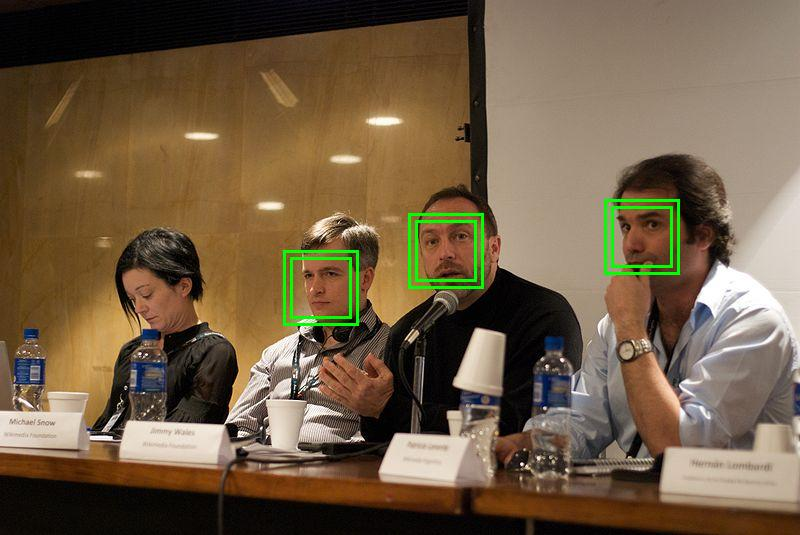
\includegraphics[width=300pt]{img2}
\caption{An example of face detection using OpenCV. Image taken from wikipedia \cite{wikiImage}}
\end{figure}

\section{Research Ideas}  \label{sec:ideas}

With the increase in popularity of cloud computing and writing applications for distributed systems, and since face detection and recognition systems built for clusters have not received much attention, our idea was to design, implement and test such a system. The goal was to think of an algorithm that would distribute work in such a way that would enable easy parallelization of the job being done, thus making it easier to be done on a cluster. Much care has been put into making it work with MapReduce programming model.

In the case of face detection, one thing this project does not deal with is classifier for deciding whether there are (and where they are) faces in a given image and we mainly focused on making the job easier by distributing the work. For the job of actually deciding whether there is a face in a given region, we employed the free-to-use solution OpenCV with its underlying Viola-Jones classifier for frontal face detection (Fig. 1 shows result of detecting faces with OpenCV). Of course, any other tool can be used instead of OpenCV with our generalized framework.

First, let us take a look at the way most of current face detection algorithms work. First of all, a face size is assumed. Then whole image is scanned with the fixed scan window size and for each position a classifier is used to decide whether current window location represents a face or not, possibly using heuristics to quickly discard regions which are unlikely to contain faces and in return gain on speed and lower false positive rate. Window is then scaled to different size and the process is repeated. In the end, we may end up with many rectangles which overlap a lot. Since they most likely represent the same face, such rectangles are averaged to a single rectangle. Scaling factor is usually set to value between 5\% to 10\% for a good ratio of quality and running speed. Increasing scale factor reduces number of times we scan the whole image and increases running time but then we might skip a scale that would identify a face and thus miss it. Decreasing it will improve sensitivity but also increase running time quite a lot. First way to introduce parallelization would obviously be to distribute different window sizes across multiple workers. Next idea would be to split image into subimages based on the current window size so as to split the space that needs to be scanned at each pass across multiple worker nodes.

% Meng
For face recognition part, we use Eigen Face Recognizer in OpenCV. We split the training image set to different nodes to enjoy data parallelism. For example, we have 800 labeled face images and 4 nodes, then we can deliver 200 images to each node. Every node will train an independent recognizer based on its training set. When a query face image arrives, we deliver it to every node, and every node will return a prediction result with some confidence. We reduce the feedback to report the most confident one. 

% Meng
Inspired by HIPI \cite{sweeney2011hipi}, we wanted to implement an image bundle data structure. We pack float images into the bundle and the whole bundle can be exported as a text file, which is the default file format for Hadoop, thus simplifying things for both us and the filesystem used.

\section{Problem Statement} \label{sec:problem}

Facial recognition is a problem of determining and identifying faces in images using computers. People have worked on it for decades and there has been much of improvement, mostly in last decade with the advance of digital image and video recording devices. It is a popular area of research in computer vision and has applications in surveillance systems, marketing, video recording, social networks etc.

Obvious application in security systems is real-time location and identification of people being recorded on surveillance cameras. One possible application in marketing would be to have saved preferences for faces detected by the system and to show adds that the person is the most interested in. In digital video recording, such as taking photos with your phone or camera, detecting faces helps automatically adjust focus, lighting and zoom level to better capture people on the image taken. Social networks have been deploying facial recognition algorithms to find people on images. Those are just some of the examples of usage of facial recognition algorithms already showing the importance of such systems.

When it comes to face recognition algorithms, we usually divide them in two groups. One is group of algorithms for face detection, and the other is group of algorithms for face recognition.

Face detection is a problem of determining locations and sizes of faces in input images. Output is usually a set of rectangles placed on the original image such that each rectangle contains a face.

Face recognition is a problem of identifying a given face with faces in a database. User inputs a face image and the system returns the user's identity, or the closest match if there is no ''exact match'' (some might argue that exact matches are meaningless and result should simply be a set of closest images). Some systems may always return a list of users that look similar to the one on input image. We do not provide similar face list in the implementation of our solution.

Moving to distributed systems (clouds), problem of face detection and recognition we deal with is how to organize input data so as to enable easy parallelization and distribution of work, retaining or gaining on speed and moving a step closer to having a fully working, efficient both in speed and space and traffic consumed and an easy to use solution. In the next section we describe the proposed solution and then show the results of our evaluation of the framework using OpenCV.

\section{Proposed Solution} \label{sec:solution}

\subsection{Face Detection}

\begin{wrapfigure}{r}{0.55\textwidth}
\centering
\includegraphics[height=300pt]{faceDetection1}
\caption{Diagram of the face detection framework. First, input image is split into many subimages and they are given as input to MapReduce.}
\end{wrapfigure}

Let us first turn our attention to the problem of finding faces in images.

As indicated in previous chapter, and as it can be seen on Fig. 2, our method pre-processes input image. First parameter to detection part is face size. Since faces on the image can be of any size, we need to check as many as possible. The algorithm starts looking for a face of size \emph{face\_size} being set to maximum - checking whether the wole image is one big face. It then scales down \emph{face\_size} and partitions the image into blocks accordingly (refer to Fig. 3).

\begin{figure}[t!]
\centering
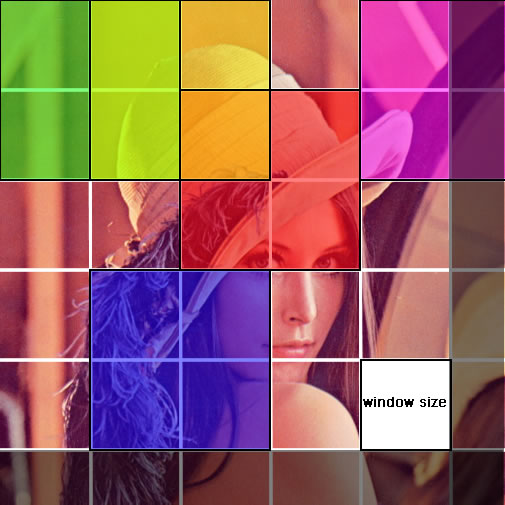
\includegraphics[width=300pt, height=300pt]{img1}
\caption{An illustration of image partitioning given the window size (assumed face size). Mesh with white lines is the cut based on window size. Green, yellow, red, purple and blue boxes represent examples of different scan areas. Scan areas overlap to make sure we don't miss any face on the boundary. Gray-shaded region represents parts of the image that cannot contain a face alone, because they are smaller than assumed face size.}
\end{figure}

We then treat all macroblocks (accross all different face sizes) consisting of 4 neighbouring blocks as potential search areas that are fed as input to classifier. Since macroblocks have width and height $2 \cdot face\_size$ every face must be contained in at least one macroblock, so classifier will not miss it. In our implementation, to ensure that there happen no repetitions of scanned regions due to scaling in OpenCV's algorithm, we fixed the size of face each time we ran the classifier. That improved running time but then we had to be careful with scaling and partitioning to ensure that we do not miss anything OpenCV would otherwise find if inner scaling was allowed.

After mapping is done and faces are detected, output is a collection of rectangles. Many of those rectangles may overlap quite a lot indicating they represent same face identified at different scale of $face\_size$ and from different macroblocks. Thus we need to do a post-processing step to find all such clusters of rectangles and average them out. It can be done by a simple line sweep algorithm; sort rectangles and scan them from left to right and top to bottom, replacing clusters of overlapping rectangles with a single one. That way we remove redundancy in the output. 

\begin{figure}
\centering
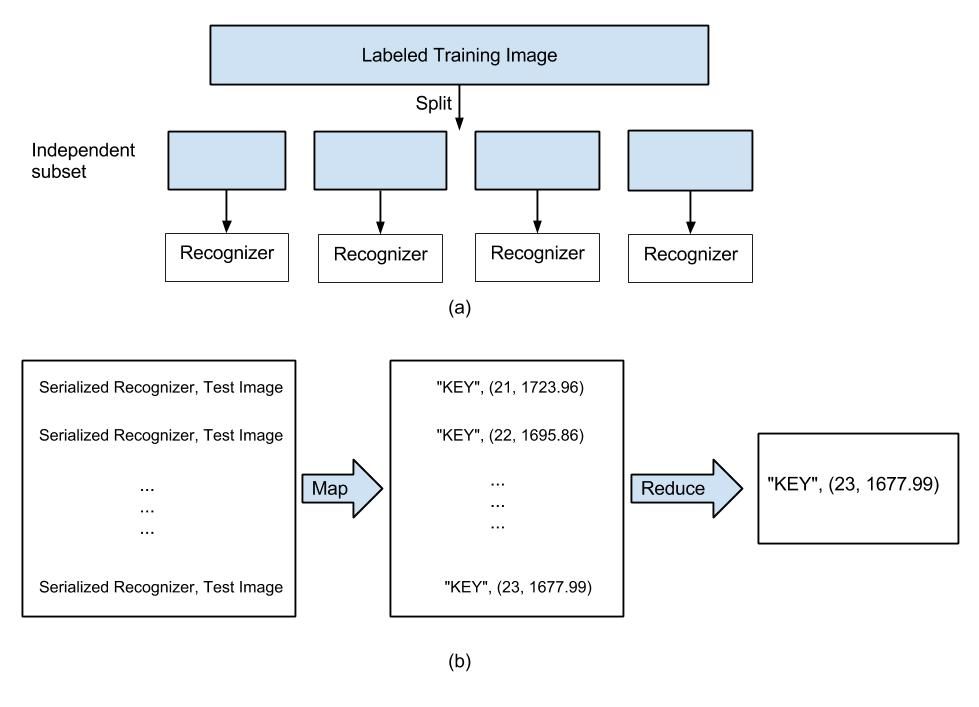
\includegraphics[height=300pt]{recog_overview}
\caption{Distributed face recognition. (a) The training set is split so that every computing node has its own training data. Independent classifiers are trained in the trainning stage. (b) When a test image arrives, we generate the input file for hadoop (the leftmost rectangle). It contains serialized classifier, which contains all the required data to make a prediction, and the test image itself. Every line of the input file is distributed to a different mapper as input, and the output will be the prediction result, in (prediction, confidence) pair. Reducers and Combiners will take these outputs to find the most confident result.}
\label{fig:recog_overview}
\end{figure}

\subsection{Face Recognition}

For face recognition, the idea is to assign training images to different nodes, so that each computing node can make its own prediction, in parallel (refer to Fig. \ref{fig:recog_overview}). 

In the training phase, we split the training data into several folds, and each fold will generate an independent recognizer. We can dump these recognizers to file system. Then, in the testing phase, when a new test image comes, we generate a Hadoop input file. This file contains the recognizers and the test image in each line, which will be distributed to each mapper later on. Every mapper will load the recognizer data and make its own prediction for the test image. (Prediction, Confidence) pairs are emitted as values to the reducer. The emitted keys are always ''KEY'' so that every prediction comes to the same reducer. The reducer will combine these pairs, in the way that only the most confident one remains. We also introduce a Combiner to locally reduce mapper results.

In order to reduce data transmition, we only put the file path of recognizers in the hadoop input. All the recognizers are copied to hadoop nodes before testing.

To train independent recognizers, we use $EigenFaceRecognizer$, which analyze training images with The Principal Component Analysis (PCA). PCA will greatly reduce the dimensionality of image representation, so that we only focus on the components that account for most of the information.\cite{faceRecognizer}. The Eigenfaces method recognize face in three major steps:

1. Do PCA on training face set, and project all the training samples into PCA subspace.
2. Project the query image into the PCA subspace.
3. Finding the nearest neighbor inside PCA subspace, and determine query image’s label based on them.

The result of the first step contains all the information needed by a $recognizer$, so we dump it into the hard disk. The information includes eigenvalues, eigenvectors and projections of all training images. Some eigenfaces can be seen in Fig.\ref{fig:eigenfaces}.

\begin{figure}
\centering
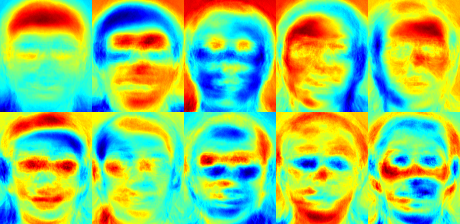
\includegraphics[height=300pt]{eigenfaces}
\caption{Trained eigenfaces. All the database images are normalized to the same size before training.}
\label{fig:eigenfaces}
\end{figure}

\begin{figure}
\centering
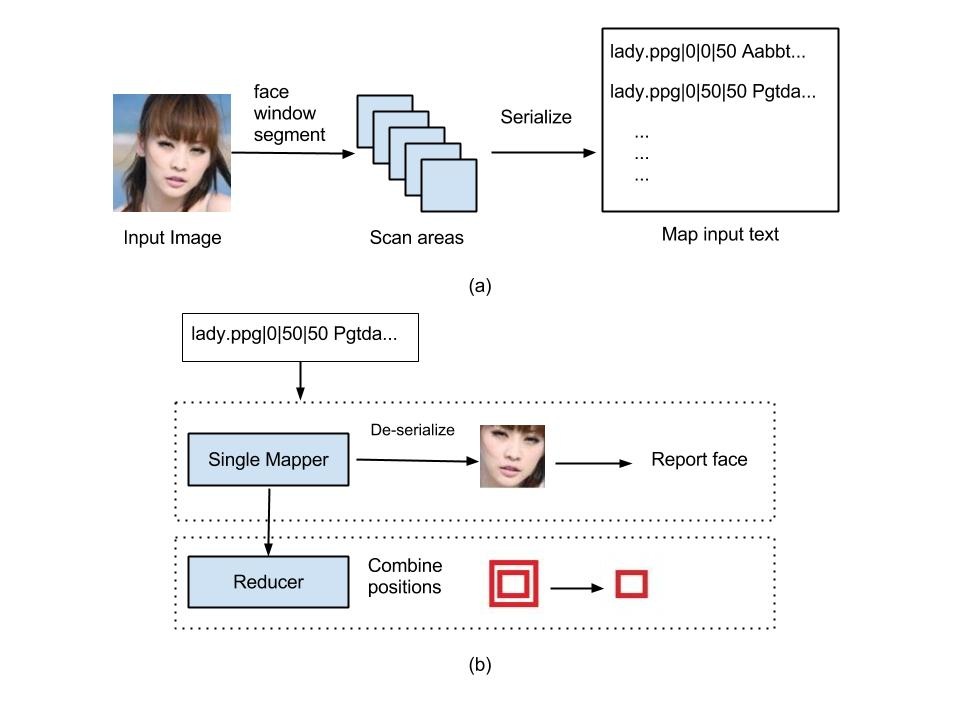
\includegraphics[height=300pt]{hadoop_face_detection}
\caption{Detailed workflow of face detection on hadoop. (a) Input image is first segmented according to different window sizes, then serialized into text string, and stored in Map input text. Filename together with window position and size are used as key. (b) Each mapper is fed with one line from the Map input text, and a sub-image can be de-serialized. We run OpenCV face detection with fixed window size on this sub-image. If there is a face, the surrounding rectangle will be emitted to reducer. The reducer merges overlapping rectangles into one.}
\label{fig:hadoop_face_detection}
\end{figure}

\subsection {General Hadoop Image Process}

Hadoop's default input and output format is text file. Although we can implement our own InputSplit and RecordReader to accommodate image input, we choose to store images as text strings. The first reason is, Hadoop's IO is only performed on disks, and its file system is not good at reading and writing many small, noncontinuous files. Instead, it's good at dealing with big files \cite{sweeney2011hipi}. After we turn every image into string, we can pack them line by line into large files, and at the same time enjoy Hadoop's default $TextInputFormat$, which will greatly reduce our programming workload. Finally, Hadoop has many hidden parameters, like the number of mappers and reducers. We believe sticking to the default file format will give us better performance, since these parameters are better tuned in default situation. We employ Base64 as the final string codec, in order to eliminate unexpected EOF or EOL inside image string.

We take face detection as an example and detailed workflow is shown in Fig. \ref{fig:hadoop_face_detection}.

\begin{figure}[t!]
\centering
\includegraphics[width=\textwidth]{segmentScales}
\caption{Subimages accross different scales. a) Example of a big window scale, not many subimages to check. b) Smaller scale of search window. Number of subimages increases exponentially. c) Smallest window scale. We have a big number of small subimages. }
\end{figure}

\section{Evaluation} \label{sec:evaluation}

In this part, we evaluate the speed of face detection and recognition. The accuracy is not evaluated due to aim of our project to be a generalized framework allowing any classifier to be used and because it is based on how well OpenCV handles small search windows with fixed scale.

The solutions have been tested on both Hadoop local filesystem and on Amazon cloud. Implementation was done using JavaCV (java version of OpenCV). For face detection, in pre-processing stage all input images are segmented across different face sizes and stored in a collection input text file. In mapping stage of face detection, subimages were read with filename, coordinates and dimensions as keys and string encoding of the image as value. On each subimage, OpenCV's Haar classifier method was invoked to find faces with fixed window size. Mapping output is filename as key and coordinates of rectangles (with offsets relative to original unsegmented image) that contain faces as values. In reduce stage, all rectangles that belong to same image are grouped due to having same key, ready to be post-processed by rectangle-averaging algorithm to remove redundancy in output rectangles.

Average running time on local Hadoop Mapreduce for a single image is around 28 seconds and for 10 images it is 65 seconds, giving us average time of roughly 4 seconds per image ignoring time spent on initialization of nodes and starting the job. On Amazon EMR, using one master node and 5 small worker nodes, time spent on processing single image was around 96 seconds, while time spent on processing 10 images was around 140 seconds

The biggest drawback of the face detection framework are repetitions. For each image and each window size, subimages were generated according to partition based on window size. As can be easily seen on Fig. 5, this introduces a lot of repeated segments of the image being copied over and over. Since there are $\log_{scaleFactor}{imageSize}$ different window sizes and almost all windows are repeated in 4 scan areas, given a fixed window size, there is approximately $O(\frac{imageSize}{minimumWindowSize})^{2} $ subimages, which is a lot. With scale factor 1.05 and minimum window size 25, more than 100MB big input file is generated for an image of size 650x500.

FDSegment: 1pic: 187MB, 95.66s; 4 pic: 870MB, 111.11s; 10 pic: 1.7GB, 140.37s (1 master, 5 core); 64.94s (local hadoop)
FRDist: 2 core: 69.92s, 4 core: 85.66s
Raw opencv face detection: 12.75s/100pics , Amazon raw face detection: 51s/5pics

\section{Conclusions and Future Work} \label{sec:conclusion}

What are the lessons that we should learn from this paper? 
What are the possible extensions of this work?


%%% The References (are kept in a separate file "refs.bib" in this example. 
\bibliographystyle{IEEEtran}   
\bibliography{./refs}    % refs.bib --> should contain all references


\end{document}

